\section{Experiment 3 : Improve Relevance Distribution}
The results from previous experiment are a strong evidence that better structured cell architecture leads to better explanation. However, there are some cases that the purposed architectures fail to distribute relevance properly.  \addfigure{\ref{fig:rel_failed_cases}} shows such cases. \todo{Here ... should not propagate relevances to .... }

\begin{figure}[h]
\centering
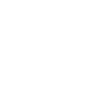
\includegraphics[draft,width=0.5\textwidth]{/sketch/placeholder}
\caption{Heatmaps of failed cases} 
\label{fig:rel_failed_cases}  %todo : figure failed cases
\end{figure}

Given the motivation above, this experiment aims to extend the proposed architectures further to better address the problem. More precisely, there are 3 improvement proposals considered here, namely stationary dropout, employing gating units,  and literal connections.

\subsection{Proposal 1 :  Stationary Dropout}
Dropout is a simple regularization technique that randomly suspends activity of neurons during training. This randomized suspension allows the neurons to learn more specific representations and reduces chance of overfitting.  It is also directly related to explanation quality. Figure .. shows explanations of LeNet trained with different dropout probability. 

\begin{figure}[h]
\centering
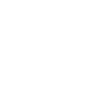
\includegraphics[draft,width=0.5\textwidth]{/sketch/placeholder}
\caption{LeNet with various dropout values} 
\label{fig:lenet various dropout}  %todo : figure failed cases
\end{figure}

However, unlike typical feedforward architectures, some RNN layers are reused across time step, hence a question arises whether the same neurons in those layers should be suspended or they should be different neurons. \addfigure{\ref{fig:lstm_naive_dropout}} and \addfigure{\ref{fig:lstm_variational_dropout}} illustrates these 2 different approaches where different colors represent different dropping activities. In particular, this stationary dropout was first proposed by \cite{GalTheoreticallyGroundedApplication2016} who applied  the technique to LSTM and GRU and found improvements on language modeling tasks.

\begin{figure}
\centering
\subfloat[Naive Dropout]{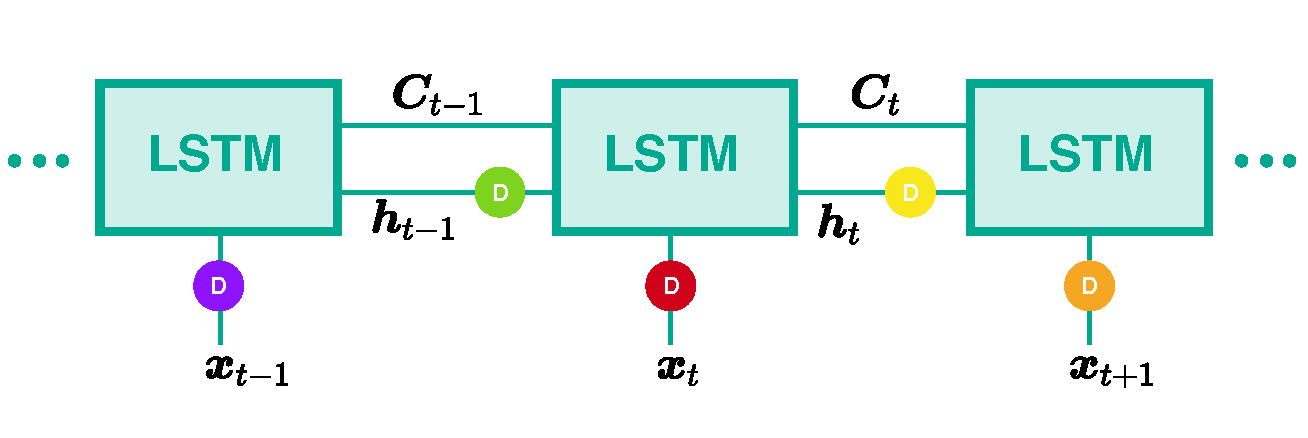
\includegraphics[width=0.8\textwidth]{sketch/lstm_naive_dropout} \label{fig:lstm_naive_dropout}} \\
\subfloat[Stationary Dropout]{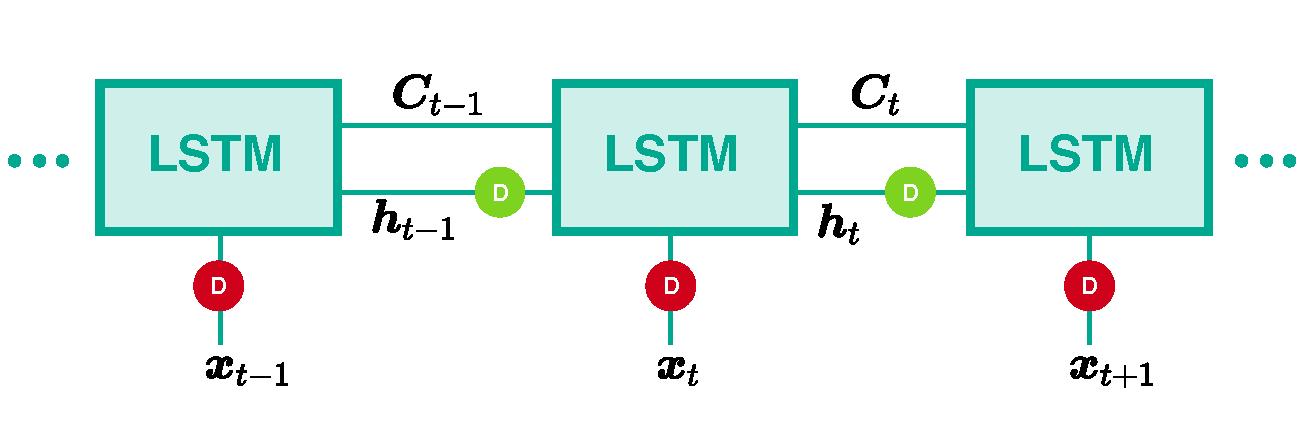
\includegraphics[width=0.8\textwidth]{sketch/lstm_variational_dropout} \label{fig:lstm_variational_dropout}}

\end{figure}

\subsection{Proposal 2 : Gating units}
It is already shown that gating units and addictive updates are critical mechanisms that enable LSTM to learn long term dependencies \cite{GreffLSTMsearchspace2017, Jozefowiczempiricalexplorationrecurrent2015a}. However, LSTM is not readily applicable for methods we are considering in this thesis. More precisely, the use of sigmoid and tanh activations violates the assumption of GB and DTD. Therefore, we propose a slight modified version of LSTM where ReLU activations are used to compute cell state candidates $\widetilde{C}_t$ instead of tanh functions. This results $C_t \in \mathbb{R}^+$, hence the tanh activation for $h_t$  is also removed.  From the following, we will refer this architecture as R-LSTM to differentiate from the original.  \addfigure{\ref{fig:relu_lstm}} presents an overview of R-LSTM architecture.

\begin{figure}[h]
\centering
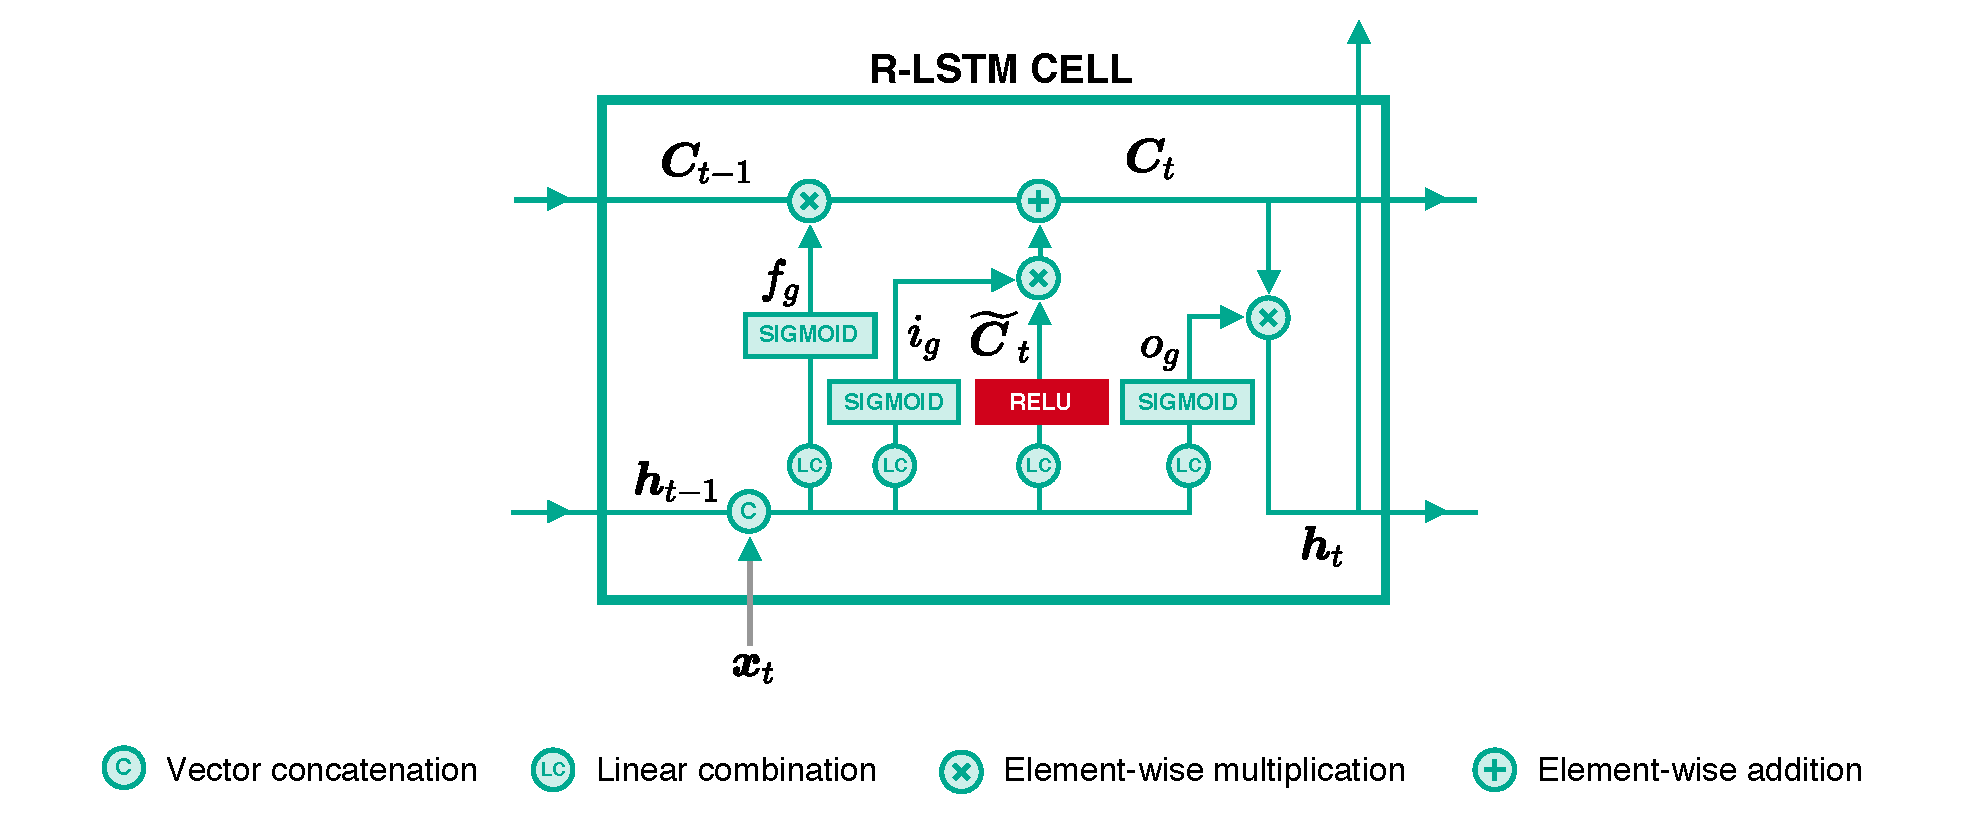
\includegraphics[width=1\textwidth]{sketch/relu_lstm}
\caption{R-LSTM Structure} 

\label{fig:relu_lstm} 
\end{figure}



%
%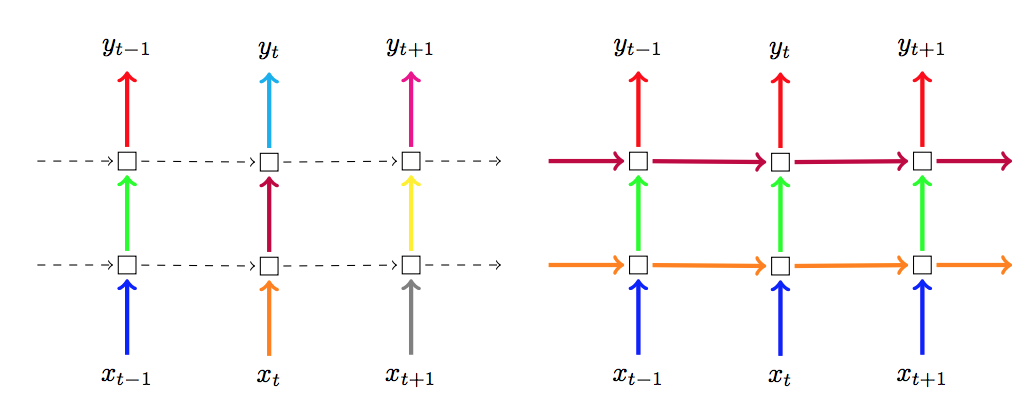
\includegraphics[width=0.7\textwidth]{variational_dropout}
%\caption{Variational Dropout\cite{GalTheoreticallyGroundedApplication2016}}
%\label{fig:variational_dropout}

\subsection{Proposal 3 : Convolutional layer with literal connections}


 \begin{figure}[h]
\centering
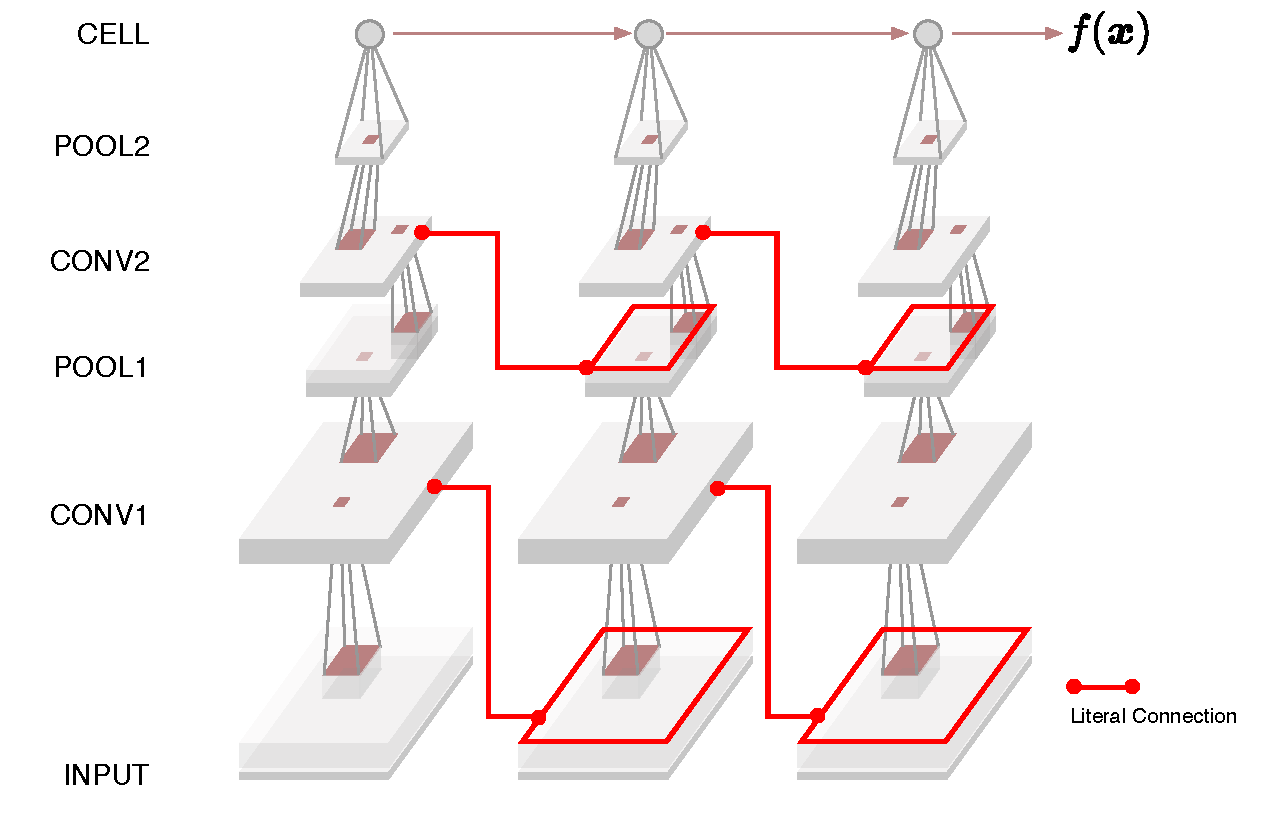
\includegraphics[width=0.7\textwidth]{sketch/conv_literalconn}
\caption{ConvDeep with Literal connections} 
\label{fig:conv_literalconn}
\end{figure}

\subsection{Result}

\subsection{Summary}